\documentclass[titlepage,dvipdfmx]{jarticle}
\usepackage[dvipdfmx]{graphicx}
\usepackage{pdfpages}
\usepackage{listings}
\usepackage{here}
\usepackage{amsmath}
\newcommand{\className}{\textbf}%\className{}で{}内の文字を太字にする処理
%
\lstset{
  basicstyle={\ttfamily},
  identifierstyle={\small},
  % commentstyle={\smallitshape},
  keywordstyle={\small\bfseries},
  ndkeywordstyle={\small},
  stringstyle={\small\ttfamily},
  frame={tb},
  breaklines=true,
  columns=[l]{fullflexible},
  numbers=left,
  xrightmargin=0zw,
  xleftmargin=3zw,
  numberstyle={\scriptsize},
  stepnumber=1,
  numbersep=1zw,
  lineskip=-0.5ex,
  language=c
}
\renewcommand{\lstlistingname}{ソースコード}
\makeatletter
\newcommand{\figcaption}[1]{\def\@captype{figure}\caption{#1}}
\newcommand{\tblcaption}[1]{\def\@captype{table}\caption{#1}}
\makeatother
\begin{document}
\section{目的}
Gameプログラムの開発を通して、オブジェクト指向プログラミングに関する技術を習得する。
\section{システムの概要}
%・新キャラクタの動作をわかりやすく記述してください。
私が作成した新キャラクターは隠しブロックである.このキャラクターは最初は現れておらず,隠しブロックがある場所にPlayerが上向きの慣性をもった状態で衝突することで出現する.
出現時,Playerは隠しブロックより上に行くことはせず,速度を失い落ちていく.それと同時にPlayerはスコアを20手に入れる.
出現後はPlatformと同じようにPlayerが下向きの慣性を持っている状態でnewCharacterに衝突することでPlayerがジャンプする.
また,出現時は図\ref{newCharacter}のような姿をしている.
\begin{figure}[H]
  \centering
  
\includegraphics[width=6cm]{img/new_character.png}
  \caption{新キャラクター出現時イメージ}
  \label{newCharacter}
\end{figure}
\section{システムの構成}
% ・新キャラクタ、および新キャラクタと関連を持つキャラクタをクラス図で示し、
% 新キャラクタの属性、メソッド、および他のキャラクタとの関係を
% わかりやすく説明してください。
新キャラクターの関係図を図\ref{class}に示す.
\begin{figure}[H]
  \centering
  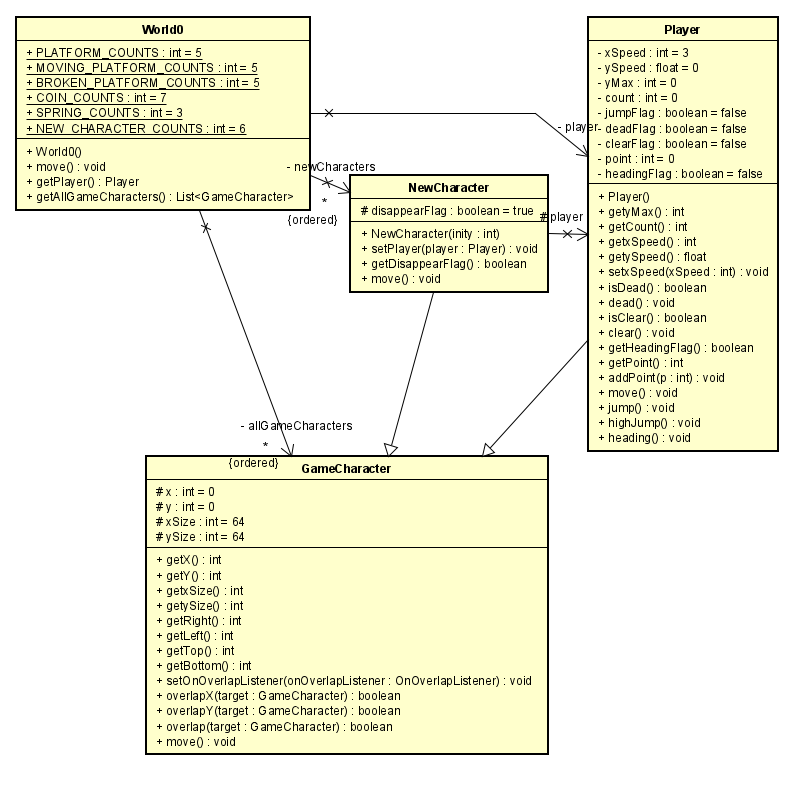
\includegraphics[width=12cm]{img/class.png}
  \caption{新キャラクタークラス図}
  \label{class}
\end{figure}

新キャラクターを定義するクラス\className{NewCharacter}は,\className{GameCharacter}を継承し,\className{Player},\className{World0}と接続している.
\subsection*{属性}
新キャラクターは\className{GameCharacter}から継承したものも含め,ソースコード\ref{property}に示すようなカプセル化が行われた属性を持っている.
\begin{lstlisting}[caption=属性,label=property]
  int x;
  int y;
  int xSize;
  int ySize;
  boolean disappearFlag;
  Player player;
\end{lstlisting}

x,y,xSize,ySizeは\className{NewCharacter}のオブジェクトの位置と大きさの定義である.

disappearFlagは\className{NewCharacter}のオブジェクトがプレイヤーの画面から隠れているか否かを管理する変数で,trueの時隠れていてfalseで出現している.
初期値はtrueである.

playerは\className{Player}と接続し利用するための変数である.

\subsection*{メソッド}
\className{GameCharacter}のメソッドをソースコード\ref{method}に示す.
\begin{lstlisting}[caption=メソッド,label=method]
public void setPlayer(Player player) {
  this.player = player;
}

public boolean getDisappearFlag(){
  return disappearFlag;
}

public void move(){
  // 隠しボックスが取得された後は足場として利用
  if(disappearFlag==false && overlap(player) == true && player.getySpeed()<0 && player.getHeadingFlag()==false){
    player.jump();
  }
  // 隠しボックスの取得
  if(getDisappearFlag()==true && overlap(player) == true && player.getySpeed()>0){//下方向から重なった場合のみ
    player.heading();
    player.addPoint(20);
    disappearFlag = false;
  }
}
\end{lstlisting}
setPlayer(),getDisappearFlag()はmove()で使うために定義したセッターとゲッターである.
move()の処理は\className{NewCharacter}のオブジェクトが\className{Player}のオブジェクトと重なった場合についての処理が記述してある.
disappearFlag=trueで隠れている場合,
\className{Player}のオブジェクトがジャンプして上向きの速度を持っている状態で
\className{NewCharacter}のオブジェクトと重なった場合にそのオブジェクトを取得するものである.
取得時の処理として,\className{Player}オブジェクトが頭をぶつける処理player.heading(),
スコアが20加算される処理player.addPoint(20),
\className{NewCharacter}のオブジェクトが叩かれたことにする処理を行っている.

% 隠蔽時の処理について
heading()は隠れている\className{NewCharacter}のオブジェクトを叩いた\className{Player}のオブジェクトが接触し,
\className{NewCharacter}のオブジェクトが出現した後すぐにジャンプしてしまったため\className{Player}に作成したメソッドである.
このメソッドをソースコード\ref{heading}に示す.
\begin{lstlisting}[caption=heading(),label=heading]
private boolean headingFlag = false;
public void heading(){
  headingFlag = true;
  ySpeed = 0.0f;
}
\end{lstlisting}

このメソッドは呼び出された時にheadingFlagを上げ,\className{Player}のオブジェクトのy軸方向のスピードを0にする処理出できている.
headingFlagは\className{Player}のオブジェクトがジャンプしたときに下ろされる様になっており,前述の問題を解決している.
なお,ばねによるハイジャンプでは解除されない仕様になっている.

% 出現時の処理について
次に,disappearFlag=falseで出現している場合,
\className{Player}のオブジェクトが\className{NewCharacter}のオブジェクトに触れて出現した後,
一回以上ジャンプした上で\className{Player}のオブジェクト自身が下向きの速度を持っている状態で,
\className{NewCharacter}のオブジェクトと重なった場合にそのオブジェクトでジャンプするものである.
\section{考察}
% ・今回のGame プログラム作成を踏まえて、以下を記述してください。
% ①オブジェクト指向プログラミングの長所
% ②オブジェクト指向プログラミングで注意すべき点
\subsection{オブジェクト指向プログラミングの長所}
オブジェクト指向プログラミングでは継承と多態性により,似たようなオブジェクトを複数作る際にクラス内のメンバやメソッドを共通化し,少ない記述量で作成できる.
また,各クラスに役割を分割することで,エラーが起きた際にエラー内容から原因のファイルが推測しやすくなる.
\subsection{オブジェクト指向プログラミングで注意すべき点}
オブジェクト指向プログラミングでは設計が重要だが,設計を過剰に複雑化しすぎると,チームの仲間や未来の自分がコードの理解や保守が難しくなり時間がかかってしまう.
オブジェクト指向プログラミングの利点をうまく利用できれば保守性や拡張性に優れたソフトウェアを開発できる反面,
上手く扱えなければそれがバグの温床になったり可読性の低下などマイナスに働きかねない.
\section{感想}
% ※ここは採点の対象外です。
% 今回の実験の内容について感想などあれば記述して下さい。
% 次年度以降の実験の実施に役立てたいと思います。
聞き逃してしまったときに解説しているスライドが配布されていない時がたまにあったのが不便だった.
今回初めて1からアプリ開発をしたが,順序立てて少しずついろいろな機能を追加していったので,オブジェクト指向についてよく学べたと思う.
\end{document}